% !TeX spellcheck = en_GB
% !TeX program = lualatex
%
% v 2.3  Feb 2019   Volker RW Schaa
%		# changes in the collaboration therefore updated file "jacow-collaboration.tex"
%		# all References with DOIs have their period/full stop before the DOI (after pp. or year)
%		# in the author/affiliation block all ZIP codes in square brackets removed as it was not %         understood as optional parameter and ZIP codes had bin put in brackets
%       # References to the current IPAC are changed to "IPAC'19, Melbourne, Australia"
%       # font for ‘url’ style changed to ‘newtxtt’ as it is easier to distinguish "O" and "0"
%
\documentclass[a4paper,
               %boxit,        % check whether paper is inside correct margins
               %titlepage,    % separate title page
               %refpage       % separate references
               %biblatex,     % biblatex is used
               keeplastbox,   % flushend option: not to un-indent last line in References
               %nospread,     % flushend option: do not fill with whitespace to balance columns
               %hyphens,      % allow \url to hyphenate at "-" (hyphens)
               %xetex,        % use XeLaTeX to process the file
               %luatex,       % use LuaLaTeX to process the file
               ]{jacow}
%
% ONLY FOR \footnote in table/tabular
%
\usepackage{pdfpages,multirow,ragged2e} %
\usepackage{physics}
%
% CHANGE SEQUENCE OF GRAPHICS EXTENSION TO BE EMBEDDED
% ----------------------------------------------------
% test for XeTeX where the sequence is by default eps-> pdf, jpg, png, pdf, ...
%    and the JACoW template provides JACpic2v3.eps and JACpic2v3.jpg which
%    might generates errors, therefore PNG and JPG first
%
\makeatletter%
	\ifboolexpr{bool{xetex}}
	 {\renewcommand{\Gin@extensions}{.pdf,%
	                    .png,.jpg,.bmp,.pict,.tif,.psd,.mac,.sga,.tga,.gif,%
	                    .eps,.ps,%
	                    }}{}
\makeatother

% CHECK FOR XeTeX/LuaTeX BEFORE DEFINING AN INPUT ENCODING
% --------------------------------------------------------
%   utf8  is default for XeTeX/LuaTeX
%   utf8  in LaTeX only realises a small portion of codes
%
\ifboolexpr{bool{xetex} or bool{luatex}} % test for XeTeX/LuaTeX
 {}                                      % input encoding is utf8 by default
 {\usepackage[utf8]{inputenc}}           % switch to utf8

\usepackage[USenglish]{babel}

%
% if BibLaTeX is used
%
\ifboolexpr{bool{jacowbiblatex}}%
 {%
  \addbibresource{jacow-test.bib}
  \addbibresource{biblatex-examples.bib}
 }{}
\listfiles

%%
%%   Lengths for the spaces in the title
%%   \setlength\titleblockstartskip{..}  %before title, default 3pt
%%   \setlength\titleblockmiddleskip{..} %between title + author, default 1em
%%   \setlength\titleblockendskip{..}    %afterauthor, default 1em

\begin{document}

\title{Electrostatic deflector Nuclotron modernization\\ for EDM experiment}

\author{S. Kolokolchikov\textsuperscript{1,2}, Y. Senichev\textsuperscript{1,2}, A. Aksentyev\textsuperscript{1,2,3}, A. Melnikov\textsuperscript{1,2,4},\\ P. Palamarchuka\textsuperscript{1,3}, E. Syresin\textsuperscript{5}, V. Ladygin\textsuperscript{5} \\
\textsuperscript{1}Institute for Nuclear Research of the Russian Academy of Sciences, Moscow, Russia\\
\textsuperscript{2}Moscow Institute of Physics and Technology, Dolgoprudny, Russia\\
\textsuperscript{3}National Research Nuclear University MEPhI, Moscow, Russia\\
\textsuperscript{4}Landau Institute for Theoretical Physics, Chernogolovka, Russia\\
\textsuperscript{5}Joint Institute for Nuclear Research, Dubna, Russia\\}
	
\maketitle

%
\begin{abstract}

	\par Considered the current Nuclotron structure for precision EDM-experiments as an independent synchrotron storage ring equipped with electrostatic deflectors. In this regard, the design should ensure the preservation and precise control of spin dynamics stability. Moreover the initial purpose of the structure as a booster of polarized beams in the collider has been preserved.

\end{abstract}

\section{Quasi-frozen spin at periodic lattice}\label{sec.II}

\par For an ensemble of particles, the spin can be described as a classical spin vector and its dynamics in external electromagnetic fields is described by the Thomas-Bargmann-Michel-Telegdi (T-BMT) equation \cite{TBMT}

\begin{equation}
	\begin{aligned}
		\dv{\vec{\mathrm{S}}}{t} = & \left(\vec{\Omega}_{\text{MDM}}+\vec{\Omega}_{\text{EDM}}\right)\times\vec{\mathrm{S}}, \\
		\vec{\Omega}_{\text{MDM}}  = & - \frac{q}{m \gamma}\left\{(\gamma G+1) \vec{\mathrm{B}}_{\perp}+(G+1) \vec{\mathrm{B}}_{\|}-\right. \\
		& \left.-\left(\gamma G+\frac{\gamma}{\gamma+1}\right) \frac{\vec{\beta} \times \vec{\mathrm{E}}}{c}\right\}, \\
		\vec{\Omega}_{\text{EDM}}  = & - \frac{q \eta}{2 m}\left(\vec{\beta} \times \vec{\mathrm{B}}+\frac{\vec{\mathrm{E}}}{c}-\frac{\gamma}{\gamma+1}\frac{\vec{\beta}}{c}\left(\vec{\beta}\cdot\vec{E}\right)\right),
	\end{aligned}
	\label{eq:T-BMT}
\end{equation}

\noindent where $\vec{\Omega}_{\text{MDM}}, \vec{\Omega}_{\text{EDM}}$ -- are precession frequency due to magnetic and electric dipole moments, $\vec{\mathrm{E}}, \vec{\mathrm{B}} = \vec{\mathrm{B}}_{\perp} + \vec{\mathrm{B}}_{\|}$ -- external magnetic and electric field. $m, q$ -- mass and charge of a particle, $\gamma$ is the Lorentz factor. The dimensionless $\eta$ factor is connected to the EDM value $d$ and the spin $s$ of a particle: $d = \frac{\eta g}{2mc}s$, $G=\frac{g-2}{2}$ -- anomalous magnetic moment. 
\par For EDM measurements, it is first necessary to compensate for MDM-effect. For this reason can be considered frozen spin method \cite{BNL}, involves an all-electric storage ring at "magic" energy for protons. This method requires the use of elements with pure electric field and the lattice must be specifically designed and operated for EDM research.
\par An alternative approach is the quasi-frozen spin concept, based on the principle of sequential spin compensation \cite{QFS}. This leads to the spin-vector oscillations back and forth relative to the momentum vector at one period and as a result at full ring.

\subsection{Relative Spin Motion at QFS}    

\par Let us introduce the concept of QFS by examining orbital and spin rotation in a generalized framework. This approach is based on the dynamics governed by the Lorentz force for orbital motion and the T-BMT equation for spin precession. It is essential to ensure first QFS condition that the orbital trajectory remains unperturbed, maintaining a closed orbit configuration

\begin{equation}
	\Phi_p^{\textrm{arc}}+\Phi_{p}^{\textrm{comp}}=\frac{2\pi}{N},\ \ \
	\label{eq:QFS_orbital}
\end{equation}

\noindent where index $p$ states for momentum, $\Phi_p^{\textrm{arc}}$ and $\Phi_{p}^{\textrm{comp}}$ -- total momentum rotation in arc and spin compensator element, $N$ is the lattice periodicity. To facilitate a lattice suitable for both EDM studies and high-energy researches, it is essential to employ a pure magnetic arc with a guiding field, given the limitations of achievable electric field strengths. In order to achieve this, a corresponding spin compensator should be implemented without perturbing the orbit. It can be formulated as $\Phi_p^{\textrm{arc}} = \frac{2\pi}{N}$, then $\Phi_{p}^{\textrm{comp}} = 0$. In order to compensate the Lorentz force, the spin compensator should utilize both magnetic and electric fields. From the Eq. \ref{eq:QFS_orbital} for spin compensation element with both magnetic and electric fields

\begin{equation}
	\Phi_{p\textrm{B}}^{\textrm{comp}}+{\Phi}_{p\textrm{E}}^{\textrm{comp}} = 0.\ \ \ 
\end{equation}

\noindent where $\Phi_{p\textrm{B}}^{\textrm{comp}}$ and ${\Phi}_{p\textrm{E}}^{\textrm{comp}}$ -- total momentum rotation in magnetic and electric fields at the spin compensator. From the T-BMT Eq.~\ref{eq:T-BMT} it can be seen that maximum effectiveness on spin electric field when it is radial to the momentum. Moreover, the momentum rotation has also the maximum value for radial electric force, which means the most effectiveness for applied field

\begin{equation}
	\vec{\Omega}_{p\mathrm{E}}^{\text{max}} = \vec{\Omega}_{p\mathrm{E}_{\perp}}=\frac{q}{m \gamma} \frac{\vec{\beta} \times \vec{\mathrm{E}}_{\perp}}{c \beta^2}
\end{equation}

\par The second condition is to compensate MDM spin rotation in one period of the ring 

\begin{equation}
	\Phi_s^{\textrm{arc}}+\Phi_{s}^{\textrm{comp}}=0,
	\label{eq:QFS_spin}
\end{equation}

\noindent where $\Phi_s^{\textrm{arc}}$ and $\Phi_{s}^{\textrm{comp}}$ -- total spin rotation in arc and spin compensator. The ratio of spin rotation relative to orbital one as follows given by spin-tune in magnetic and electric fields

\begin{equation}
	\nu_{\mathrm{B}_{\perp}} = \gamma G, \quad \nu_{\mathrm{E}} = \gamma \beta^2 \left(G-\frac{1}{\gamma^{2}-1}\right).
	\label{eq:spin-tine}
\end{equation} 

\noindent So, compensation occurs due to the fundamental difference between spin rotation in a magnetic and electric fields. And the coupling equations for pure magnetic arc $\Phi_{s}^{\text{arc}} = \nu_{\mathrm{B}_{\perp}}\Phi_{p}^{\text{arc}}$ and magnetic $\Phi_{s\mathrm{B}}^{\text{comp}} = \nu_{\mathrm{B}_{\perp}}\Phi_{p\mathrm{B}}^{\text{comp}}$, electrical $\Phi_{s\mathrm{E}}^{\text{comp}} = \nu_{\mathrm{E}}\Phi_{p\mathrm{E}}^{\text{comp}}$ field in spin compensator. Then for Eq. \ref{eq:QFS_spin}

\begin{equation}
	\begin{aligned}
		\nu_{\mathrm{B}_{\perp}}\Phi_{p}^{\text{arc}} +
		\left(\nu_{\mathrm{B}_{\perp}}\Phi_{p\mathrm{B}}^{\text{comp}} +
		\nu_{\mathrm{E}}\Phi_{p\mathrm{E}}^{\text{comp}} \right) & = \\
		= \nu_{\mathrm{B}_{\perp}} \left( 
		\Phi_{p}^{\text{arc}} +
		\Phi_{p\mathrm{B}}^{\text{comp}} \right) +
		\nu_{\mathrm{E}}\Phi_{p\mathrm{E}}^{\text{comp}}  & = 0.
		\label{eq:deflection}
	\end{aligned}
\end{equation}

\par Finally, from first and second condition can be received for rotation via magnetic or electric field in spin compensator element

\begin{equation}
	\Phi_{p\mathrm{E}}^{\textrm{comp}} = - \Phi_{p\mathrm{B}}^{\textrm{comp}} = {\Phi}_{p}^{\text{arc}}\frac{\gamma^2 G}{G+1} =\frac{2\pi}{N}\frac{\gamma^2 G}{G+1}.
	\label{eq:deflection}
\end{equation}

\noindent No mention was made of the physical structure of the compensation element, only of the integral features of the presented field components.

\subsection{Spin Compensation Element Length}

Spin compensation element length can be calculated for magnetic and electric field

\begin{equation}
	L = \Phi_{p\mathrm{B}}^{\text{comp}}R_{\mathrm{B}} = \Phi_{p\mathrm{E}}^{\text{comp}}R_{\mathrm{E}},
	\label{eq:length}
\end{equation}

\noindent where $R_{\mathrm{B}}, R_{\mathrm{E}}$ -- radius of magnetic and electric fields. In general, total radius for element with combined magnetic and electric fields can be find as

\begin{equation}
	\frac{1}{R} = \frac{1}{R_{\mathrm{B}}}+\frac{1}{R_{\mathrm{E}}}, \quad R_{\mathrm{B}}=\frac{\mathrm{B}\rho}{\mathrm{B}}, \quad R_{\mathrm{E}}=\frac{\kappa}{\mathrm{E}},    
	\label{eq:total_radius}
\end{equation}

\noindent where $\mathrm{B}\rho = \cfrac{p_{0}}{e}$ -- magnetic rigidity, $p_{0} = \gamma m\beta c$, $\kappa = \cfrac{p_{0}\beta c}{e}$ -- electrical rigidity. If we consider no orbital distortion in total, the Lorentz force should be zero, so $R=0$ and $R_{\mathrm{B}} = -R_{\mathrm{E}}$.

The limitation on the strength of the electric field is much more significant than in the case of a magnetic field. According to the Eqs. \ref{eq:deflection} and \ref{eq:length} can be received the length of compensator element per one period

\begin{equation}
	\begin{aligned}
		L_{\text{min}} = \Phi_{p\mathrm{E}}^{\text{comp}}R_{\mathrm{E}} & = 
		\frac{2\pi}{N}\frac{\gamma^2 G}{G+1}\frac{\kappa}{\mathrm{E}_{\text{max}}} = \\
		& = \frac{2\pi}{N}\frac{G}{G+1}\frac{mc^2}{e}\frac{\gamma(\gamma^2-1)}{\mathrm{E}_{\text{max}}},
		\label{eq:length_min}
	\end{aligned}
\end{equation}

\noindent where $\mathrm{E}_{\text{max}}$ -- maximum of electric field, that limit the minimal achievable length regardless the researched particle. For total length $L=L_{\text{min}}^{\text{total}} = N\cdot L_{\text{min}}$ and is independent from number of periods. Maximum attainable electric field are 10-13 MV/m \cite{wien}, this corresponds to a magnetic field of the order of 70-90 mT accordingly, it will be used later for evaluation.

\section{Electrostatic deflector}

\par Pure electrostatic deflector designed to manipulate particle trajectories and spin dynamics by creating a radial electric field with non-zero curvature. This setup is particularly useful for creating bypass sections in addition to native straight sections, allowing for flexible experimental configurations. But it requires the usage of kicker magnet to deflect beam at bypass section.

\par For EDM measurements the experiment energy 270 MeV determines by polarimeter needs \cite{pol}. Additionally, orbital and spin dynamics vary among different types of particles. First, the mass-to-charge ratio of deuterons two times more than for protons. Second, the anomalous magnetic moments are notably different: $G_{\text{p}} = 1.79$ for protons and $G_{\text{d}}~=~-0.14$ for deuterons. According to Eq. \ref{eq:deflection} the sign of rotation differs, this shows the necessity of rotating it by $\pi$ along the longitudinal axis. Additionally, the minimal achievable spin compensator length as given by Eq. \ref{eq:length_min}, is longer for proton than deuteron at optimal polarimeter energy. All these differences can be seen at Fig. \ref{fig:scheme} for various particles.

\begin{figure}[!h]
	\centering
	a. Deuteron 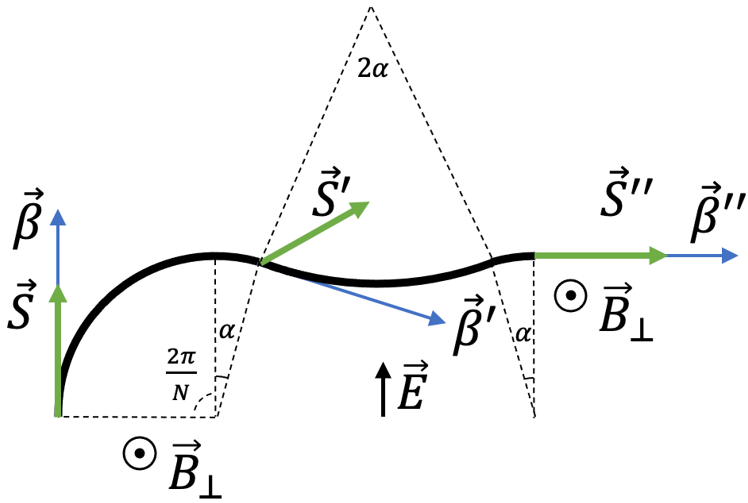
\includegraphics[width=0.8\hsize]{img/TUPS031_f1}\\
	b. Proton 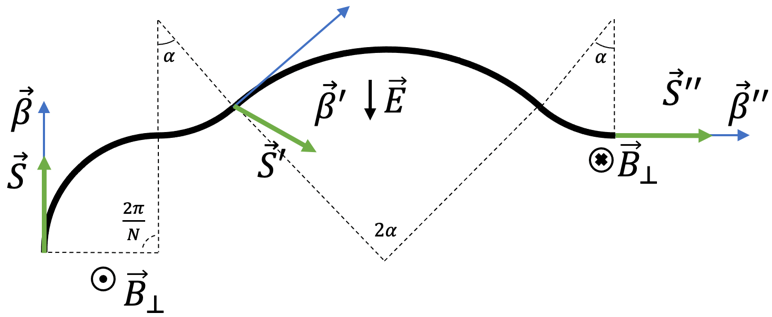
\includegraphics[width=0.95\hsize]{img/TUPS031_f2}
	\caption{A schematic diagram of a QFS structure single period with electrostatic deflector and kicker for a. deuteron and b. proton beam.}
	\label{fig:scheme}
\end{figure}

\par A primary advantage of the QFS lattice is its capacity to preserve particle acceleration at high energy range, thereby making the facility a unique instrument for diverse experimental applications. The current Nuclotron structure shown in Fig.~\ref{fig:current} is considered as а NICA collider booster and setup for fixed target experiments \cite{Nuc}. For electric field $E=13$ MV/m the total deflector length $L_{\text{el}}=53$ m for deuterons. The maximum distance is 17 cm between two beampipes: pure straight section and bypass. Which is not enough to locate both necessary equipment at straight section and deflector at bypass. For this reason other principle can be considered. 

\begin{figure}[!h]
	\centering
	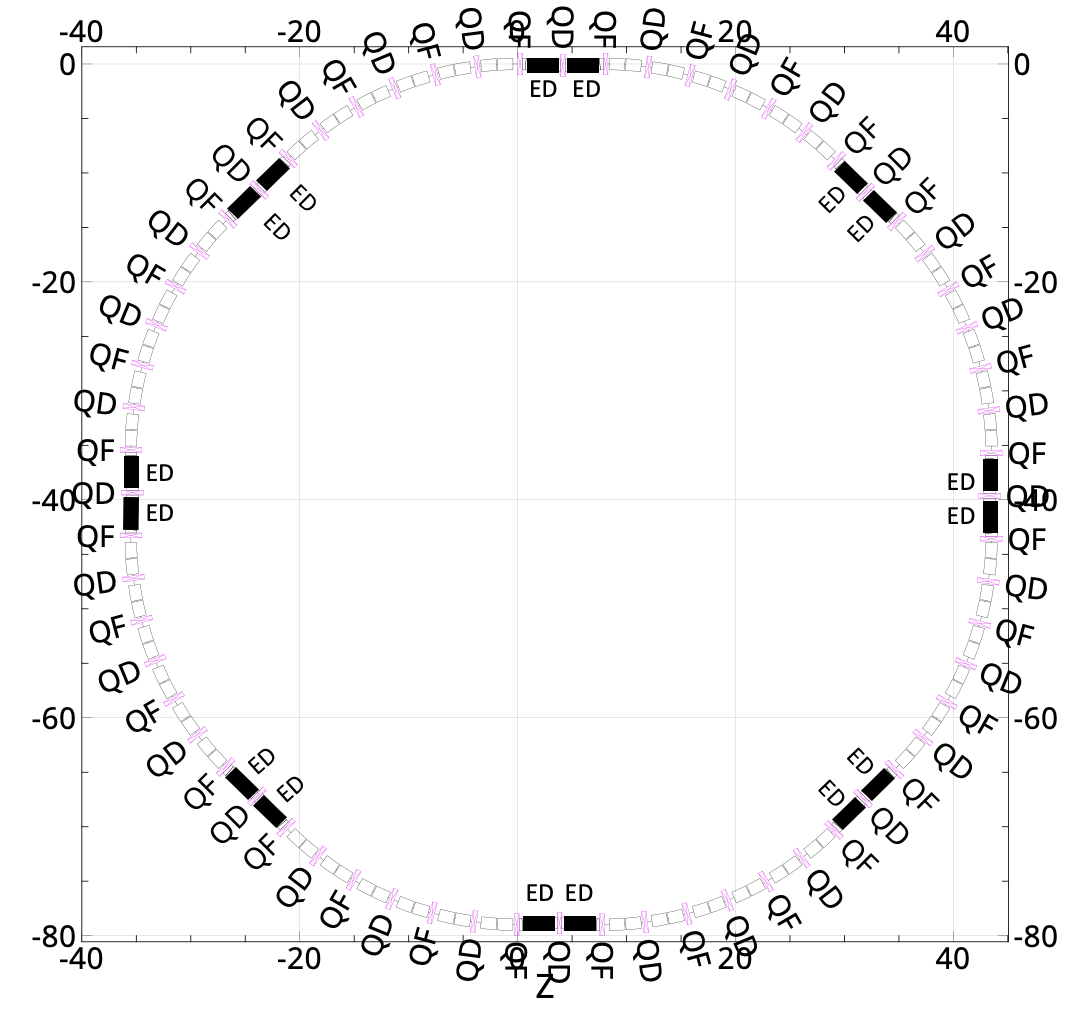
\includegraphics[width=0.9\hsize]{img/TUPS031_f3}
	\caption{Floor plan of Nuclotron's QFS lattice with electrostatic deflectors and kickers.}
	\label{fig:current}
\end{figure}

\par 

\begin{figure}[!ht]
	\centering
	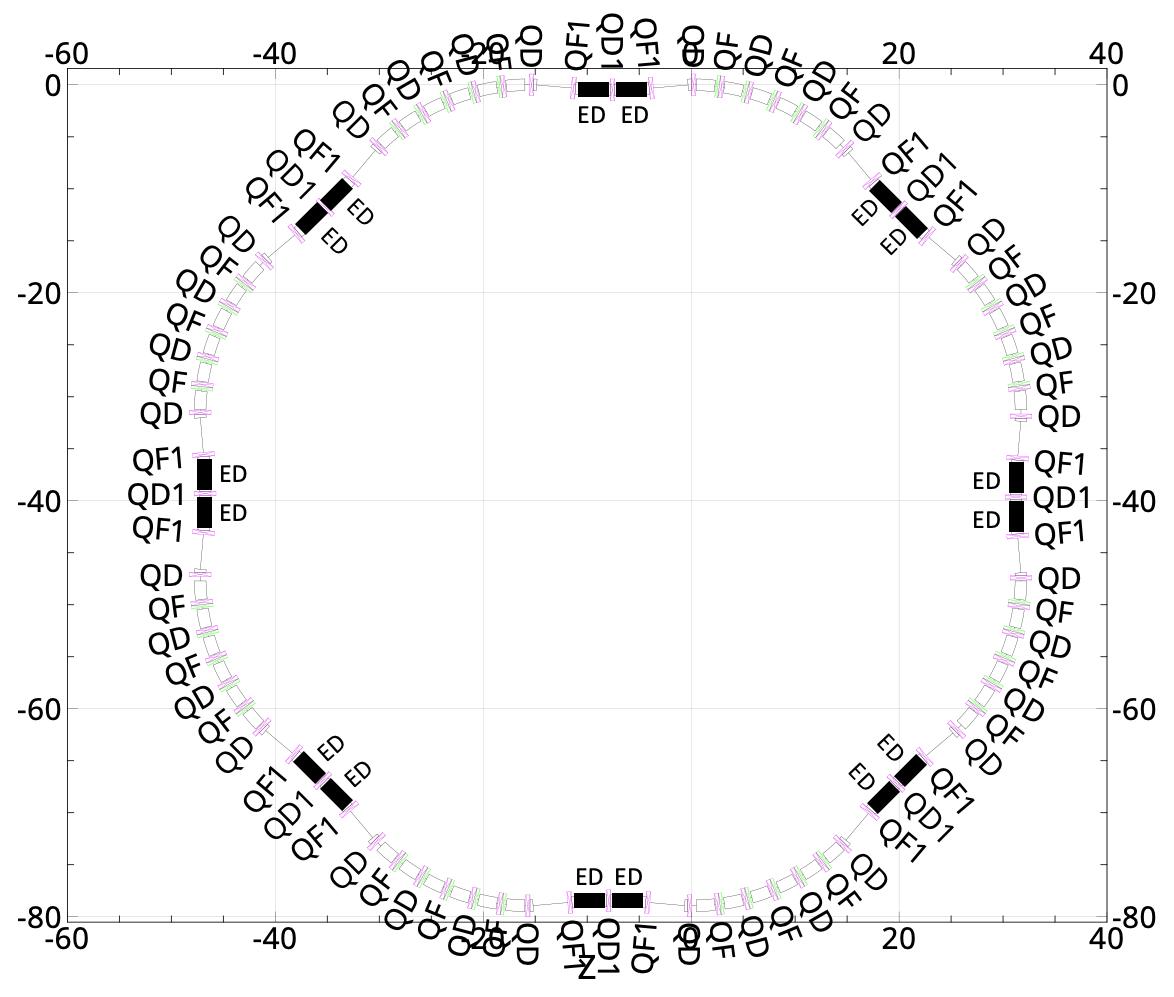
\includegraphics[width=0.9\hsize]{img/TUPS031_f4}
	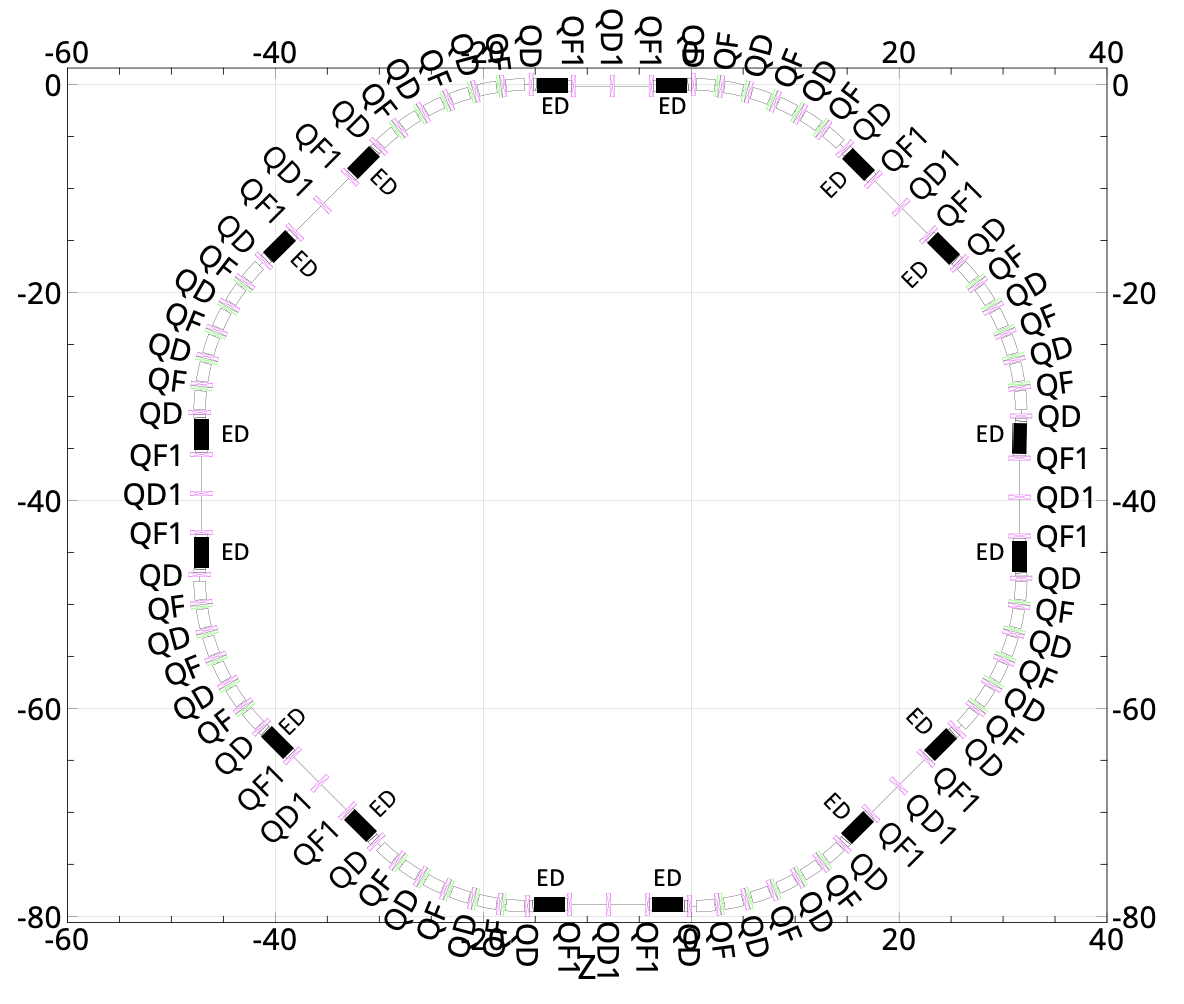
\includegraphics[width=0.9\hsize]{img/TUPS031_f5}
	\caption{Floor plans of Nuclotron's modernized QFS lattice with electrostatic deflectors and kickers.}
	\label{fig:modern}
\end{figure}

\par Modernized Nuclotron lattice is considered in order to make longer straight sections and install equipments consistently and not to overlap each other. This require to make dipole magnets shorter, here considered the transition from 1.44 to 1.8 T and total magnet length changes from 200 to 150 m accordingly. There are two ways how electrostatic deflectors can be implemented between arcs: 1) at the centre; 2) at the edges and shown at Fig. \ref{fig:modern}. The maximum distance between two beampipes are $47$ cm and $50$ cm, respectively. 

\par Despite these complexities, the electrostatic deflector with kicker offers a robust solution for controlling particle spin and trajectory. In contrast, Wien filter method can provide a great advantage in QFS lattice construction and also will represent at this conference \cite{WFmethod}.

\section{CONCLUSION}

\par This article presents the implementation of a quasi-frozen spin structure with electrostatic deflector for a periodic lattice to study the Electric Dipole Moment of charged light particles. The design achieves precise spin compensation of MDM-effect per one period by employing elements with matched curvatures for electric and magnetic fields, allowing for effective spin manipulation. An expression for the optimal spin compensator length is derived.
\par Considered the implementation of electrostatic deflector with corresponding kicker in current Nuclotron structure and a possible modernization with a high magnetic field in dipoles. The study demonstrates the versatility of the quasi-frozen spin lattice, which can be adapted for multiple purposes, including higher-energy researches within existing facilities.

\section{Acknowledgments}

\par A support of thus study by the Russian Science Foundation grant 25-72-30005 is acknowledged.

\ifboolexpr{bool{jacowbiblatex}}
	{\printbibliography}
	{
	\begin{thebibliography}{9}
	
	\bibitem{TBMT} V.Bargmann, L.Michel, V.L.Telegdi, ``Precession of the Polarization of Particles Moving in a Homogeneous Electromagnetic Field", \emph{Phys. Rev. Lett.}, vol. 2, p.~435, 1959.\\ \url{doi:10.1103/PhysRevLett.2.435}
	\bibitem{BNL} V.Anastassopoulos \emph{et al.}, ``A Storage Ring Experiment to Detect a Proton Electric Dipole Moment",  \emph{Rev.Sci.Instrum.}, vol. 87, p.~115116, 2016. \url{doi:10.1063/1.4967465}
	%\bibitem{AGS} D.Anastassopoulos et al., AGS proposal: Search for a permanent electric dipole moment of the deuteron nucleus at the $10^{-29}$ $e\cdot$cm level. \url{https://www.bnl.gov/edm/files/pdf/deuteron_proposal_080423_final.pdf}. April, 2008
	\bibitem{QFS} Yu.Senichev \emph{et al}, "Investigation of Lattice for Deuteron EDM Ring", \textit{ICAP2015 Proccedings}, pp. 17--19, 2016. \url{doi:10.18429/JACoW-ICAP2015-MODBC4}
	\bibitem{QFS} Yu. Senichev ,\textquotedblleft{Investigation of Lattice for Deuteron EDM Ring}\textquotedblright, in \emph{Proc. ICAP2015}, pp. 17--19, 2016. \url{doi:10.18429/JACoW-ICAP2015-MODBC4}
	\bibitem{wien} A.Aggarwal, A.Magiera, ``Controlling Systematic Uncertainties in Search for an EDM in the Storage Ring",  \emph{Acta Phys. Pol. B}, vol. 51, p.~373, 2020. \url{doi:10.5506/APhysPolB.51.373}
	\bibitem{pol} M.W.Mcnaughton \emph{el al.}, ``The P-C Analyzing Power Between 100 MeV and 750 MeV", \emph{Nuc. Inst. and Meth. in Phys. Res. Sec. A}, vol. 241, pp.~435-440, 1985.\\ \url{doi:10.1016/0168-9002(85)90595-9}
	\bibitem{Nuc} 
	A. D. Kovalenko \emph{et al.},
	\textquotedblleft{Nuclotron at JINR: Operation Experience and Recent Development}\textquotedblright,
	in \emph{Proc. HIAT’15}, Yokohama, Japan, Sep. 2015, paper MOPA19, pp. 86--88.\\ \url{doi:10.18429/JACoW-HIAT2015-MOPA19}
	\bibitem{WFmethod}
	 Y. Senichev \emph{et al.},
	 \textquotedblleft{Wien filter method for the "Quasi-frozen" spin lattice}\textquotedblright,
	 presented at the IPAC’25, Taipei, Taiwan, Jun. 2025, paper TUPS032, this conference.  
	
	\end{thebibliography}
}

\end{document}